% --------------------------------------------------------------------

\chapter[Cosmology]{Accurate Cosmological Measurements on the Largest Scales}
\def\chpname{cosmo}\label{chp:\chpname}

Chapter editors:
\credit{egawiser},
\credit{MichelleLochner}.

Contributing authors:
\credit{tanguita},
\credit{HumnaAwan},
\credit{rbiswas4},
\credit{PeterKurczynski},
\credit{drphilmarshall},
\credit{jmeyers314},
\credit{jhrlsst}.

% --------------------------------------------------------------------

\section{Introduction}
\label{sec:\chpname:intro}

Cosmology is one of the key science themes for which LSST was
designed. Our goal is to measure cosmological parameters, such as the
equation of state of dark energy, or departures from General
Relativity, with sufficient accuracy to distinguish one model from
another, and hence drive our theoretical understanding of how the
universe works, as a whole. To do this will necessarily involve a
variety of different measurements, that can act as cross-checks of
each other, and break parameter degeneracies in any single one.

The  Dark Energy Science Collaboration (DESC) has identified five
different cosmological probes enabled by the LSST: weak lensing (WL),
large scale structure (LSS), type Ia supernovae (SN), strong lensing
(SL), and clusters of galaxies (CL). In all cases, the primary concern
is residual systematic error: the shapes and photometric redshifts of
galaxies, and the properties of supernova and lensed quasar light
curves, will all need to be measured with extraordinary accuracy in
order for LSST's high statistical power to be properly harnessed. This
accuracy will come from the abundance and heterogeneity of the
individual measurements made, and the degree to which they can be
modeled and understood. This latter point implies a need for uniformity
in the survey, which enables powerful simplifying assumptions to be made
when calibrating on the largest, cosmologically most important scales.
The need for heterogeneity also implies  uniformity, in the sense that
the nuisance parameters that describe the systematic effects need to be
sampled over as wide a range as possible (examples include the need to
sample a wide range of roll angles to minimize shape error, and
observing conditions to understand photometric errors due to the
changing atmosphere).

In this chapter we look at some of the key measurements planned by the
Dark Energy Science Collaboration, and how they depend on the
Observing Strategy.


%---------------------------------------------------------------------

% ====================================================================
%+
% SECTION NAME:
%    lss.tex
%
% CHAPTER:
%    cosmology.tex
%
% ELEVATOR PITCH:
%    Large Scale Structure, Weak Lensing, and Clusters all require
% survey uniformity in the static 10-year survey.  A key contributor to 
%this is the pattern of dithers adopted.  
%
% COMMENTS:
%
%
% BUGS:
%
%
% AUTHORS:
%   Eric Gawiser (@egawiser)
%-
% ====================================================================
\clearpage
\section{Large Scale Structure:  Testing Dithering Patterns and Timescales to Improve Survey Uniformity}
\def\secname{lss}\label{sec:\secname}

\noindent{\it Humna Awan, Eric Gawiser, Peter Kurczynski, Lynne Jones} % (Writing team)

% This individual section will need to describe the particular
% discoveries and measurements that are being targeted in this section's
% science case. It will be helpful to think of a ``science case" as a
% ``science project" that the authors {\it actually plan to do}. Then,
% the sections can follow the tried and tested format of an observing
% proposal: a brief description of the investigation, with references,
% followed by a technical feasibility piece. This latter part will need
% to be quantified using the MAF framework, via a set of metrics that
% need to be computed for any given observing strategy to quantify its
% impact on the described science case. Ideally, these metrics would be
% combined in a well-motivated figure of merit. The section can conclude
% with a discussion of any risks that have been identified, and how
% these could be mitigated.

% A short preamble goes here. What's the context for this science
% project? Where does it fit in the big picture?

Three of the key cosmology probes available with LSST represent ``static science'' insensitive to time-domain concerns.  These are Weak Lensing, Large-Scale Structure, and Galaxy Clusters.  Nonetheless, due to the need to track and correct for the survey ``window function'' in all of these probes, cosmology with LSST will benefit greatly from achieving survey depth as uniform as possible over the WFD area.  OpSim tiles the sky in hexagons inscribed within the nearly-circular LSST field-of-view.  It has been shown in \citet{CarrollEtal2014} that the default LSST survey strategy implemented in OpSim runs leads to a strongly non-uniform ``honeycomb'' pattern due to overlapping regions on the edges of these hexagons receiving double the observing time.  A pattern of large dithers proves sufficient to greatly reduce these overlaps, leading to an increase in median survey depth in each filter of 0.08 magnitudes.  

In this section, we report results from an investigation by Awan et al. (in preparation) of several geometrical patterns for dithers performed on timescales varying from once per observing season to once per night to every visit.  

\todo{EG}{Flesh out WL, LSS, and Clusters dependence on survey uniformity to make this section more clearly science-driven.}  

% --------------------------------------------------------------------

\subsection{Dithering Patterns and Timescales}
\label{sec:\secname:strategies}


% --------------------------------------------------------------------

\subsection{Metrics}
\label{sec:\secname:metrics}

% Quantifying the response via MAF metrics: definition of the metrics,
% and any derived overall figure of merit.

Our primary metric is total uncertainty in the derived window function over relevant angular scales, modeled via variations in the angular power spectrum of fake galaxy fluctuations between $gri$ bands.  
Intermediate metrics include the number of galaxies in 
each pixel, fluctuations in this number, total power in the angular power spectrum of a skymap of those fluctuations, and residual power that angular power spectrum after subtracting a smooth fit to it.  



% --------------------------------------------------------------------

\subsection{OpSim Analysis}
\label{sec:\secname:analysis}

% OpSim analysis: how good would the default observing strategy be, at
% the time of writing for this science project?

In this section we present our ongoing \OpSim / MAF
analysis, as we try to
answer the question ``what dithering strategies produce acceptable variations in survey uniformity, and which appears optimal?''

%We used the
%\simsMAFcontrib{SeasonStacker}{mafContrib/seasonStacker.py} to work
%with seasons.

%We used \texttt{ops2\_1075} for most of our tests, but we need to now
%re-run on \opsimdbref{db:enigma}, and others from \autoref{chp:cadence2015}.


%\citeauthor{LiaoEtal2015}). These sky maps show that, over the main

%\autoref{tab:lenstimedelays:results} shows the global (i.e. al-sky)


%--------------------------------------------------------------------

\subsection{Results}
\label{sec:\secname:results}


\todo{EG}{Improve figures to originals rather than screen-captures.}


%%%%%%%%%%%%%%%%%%%%%%%%%%%%%%%%%
\begin{figure}[tbh!]
\vskip -0.1in
\includegraphics[angle=0,width=0.99\hsize:,clip]{figs/awan_fig1.png}
%\vskip -1.3in
\caption{}
\label{fig:seasonal_dithers}
\end{figure}
%%%%%%%%%%%%%%%%%%%%%%%%%%%%%%%%%

%%%%%%%%%%%%%%%%%%%%%%%%%%%%%%%%%
\begin{figure}[tbh!]
\vskip -0.1in
\includegraphics[angle=0,width=0.99\hsize:,clip]{figs/awan_fig2.png}
%\vskip -1.3in
\caption{}
\label{fig:nightly_dithers}
\end{figure}
%%%%%%%%%%%%%%%%%%%%%%%%%%%%%%%%%

%%%%%%%%%%%%%%%%%%%%%%%%%%%%%%%%%
\begin{figure}[tbh!]
\vskip -0.1in
\includegraphics[angle=0,width=0.99\hsize:,clip]{figs/awan_fig4.png}
%\vskip -1.3in
\caption{}
\label{fig:dithering_histograms}
\end{figure}
%%%%%%%%%%%%%%%%%%%%%%%%%%%%%%%%%

%%%%%%%%%%%%%%%%%%%%%%%%%%%%%%%%%
\begin{figure}[tbh!]
\vskip -0.1in
\includegraphics[angle=0,width=0.99\hsize:,clip]{figs/awan_fig5.png}
%\vskip -1.3in
\caption{}
\label{fig:dithering_skymaps}
\end{figure}
%%%%%%%%%%%%%%%%%%%%%%%%%%%%%%%%%

%%%%%%%%%%%%%%%%%%%%%%%%%%%%%%%%%
\begin{figure}[tbh!]
\vskip -0.1in
\includegraphics[angle=0,width=0.99\hsize:,clip]{figs/awan_fig6.png}
%\vskip -1.3in
\caption{}
\label{fig:dithering_power_spectra}
\end{figure}
%%%%%%%%%%%%%%%%%%%%%%%%%%%%%%%%%




%%%%%%%%%%%%%%%%%%%%%%%%%%%%%%%%%%%%
%\begin{figure*}[!ht]
%  \capstart
%  \begin{minipage}[b]{\linewidth}
%    \begin{minipage}[b]{0.32\linewidth}
%      \centering\includegraphics[width=\linewidth]{figs/Accuracy_season_nca.pdf}
%    \end{minipage} \hfill
%    \begin{minipage}[b]{0.32\linewidth}
%      \centering\includegraphics[width=\linewidth]{figs/Precision_cadence_nca.pdf}
%    \end{minipage} \hfill
%    \begin{minipage}[b]{0.32\linewidth}
%      \centering\includegraphics[width=\linewidth]{figs/Fraction_season_nca.pdf}
%    \end{minipage}
%  \end{minipage}
%\caption{Examples of changes in accuracy $A$ (left), precision $P$ (center) and success fraction $f$ (right) with schedule properties, as seen in the different TDC submissions. The gray
%approximate power law model was derived by visual inspection of the
%pyCS-SPL results; the signs of the indices were pre-determined according to our expectations. Reproduced from \citet{LiaoEtal2015}.}
%\label{fig:tdcresults}
%\end{figure*}
%%%%%%%%%%%%%%%%%%%%%%%%%%%%%%%%%%%


\todo{EG}{Input fuller results and text from Awan et al. draft.}  

%---------------------------------------------------------------------

\subsection{Figure of Merit}
\label{sec:\secname:fom}



\navigationbar

% ====================================================================


% --------------------------------------------------------------------

% ====================================================================
%+
% SECTION NAME:
%    wl.tex
%
% CHAPTER:
%    cosmology.tex
%
% ELEVATOR PITCH:
%-
% ====================================================================

\section{Weak Lensing}
\def\secname{wl}\label{sec:\secname}

\credit{tonytyson},
\credit{jmeyers314},
\credit{StephenRidgway}.

Much of LSST cosmology may be limited by systematic errors rather than photon
signal-to-noise. This is especially true of weak gravitational lensing,  which
relies on very accurate (\ie low bias), but very low signal-to-noise,
measurements of the shapes of galaxies, and high signal-to-noise measurements of
PSF calibration stars. As outlined in the SRD, uniformity of seeing in the bands
used for WL and special observing strategies are required in order to reduce
additive and multiplicative shear systematics.

Achieving the ultimate sensitivity of the LSST to weak lensing science places
stringent requirements on our ability to accurately measure galaxy shapes and
redshifts, which in turn demands precise and accurate knowledge of the point
spread function, astrometry, and photometry. These measurements are influenced
by the interaction of light with the Earth's atmosphere, the telescope optics,
and the CCD sensors. Sysematics in the shear are introduced in each case.
Methods have been developed for suppressing these systematics in current lensing
surveys. These and new methods will be applied to the LSST survey.

Over the sample of 3-4 billion galaxies, the shear systematics must be below one
part in 10,000 for additive shear, and one part in 1000 for multiplicative
shear. Each visit to a sky patch encounters these systematics. Some observing
strategies can effectively randomize these over all visits to a field.  Below we
discuss the observing strategies for suppressing shear systematics and metrics
for their success.

\subsection{Target Selection}

Image quality must be uniformly good in the bands used for weak lens shear.
These will be the $r$ and $i$ bands.   Depending on the current weather and
seeing, the scheduler will have a list of priorities for next-field, based on
prior history of coverage. Nearby fields in need of coverage in these bands will
be given high priority if the seeing is better than some specified value, likely
0.7 arcsec FWHM.


\subsection{Target Measurements}

It is expected that even after maximal optimization of camera optics and
electronics, that systematic image shape errors will be associated with the
orientation of the camera focal plane.  Using data from vendor CCDs, simulations
of LSST observing have shown that a combination of x-y dithering on the sky and
pipeline processing with pixel re-map (to cancel much of the CCD frame fixed
distortions) can get well within a factor of ten of the goal for shear
systematics residuals.  Simulations which add camera angle dithering show that
the goal can be achieved in fields with relatively uniform seeing history.

Thus shear systematics will be partially reduced by randomization of the
orientation of the camera with respect to the sky.  This is represented by the
parameter RotSkyPos: we can construct diagnostic metrics that quantify the
uniformity of its distribution at each sky position.   Given the spin 2 symmetry
of shear, the optimal strategy for shear systematics will be to aim for
uniformity of RotSkyPos mod $\pi$, since angles separated by $\pi$ radians are
degenerate.

Similarly, the telescope optics may harbor systematic aberrations, and these
also could be mitigated by recording images with varying parallactic angle.
Also important is the effect of atmospheric differential chromatic refraction
which act along the parallactic angle.  Re-visits to a given field should be
distributed over parallactic angles (or equivalently, hour angles), consistent
with airmass and seeing limits.

Uniformity of depth is important, but less so than uniformity in camera rotator
shear suppression.  Simulations have shown that for the Gold sample of galaxies,
uniformity at the 0.2 mag level in limiting magnitude produces little shear
bias. The largest effect comes from bias in weak lens magnification tomography.


\subsection{Metrics}

For characterizing the isotropy of rotational sampling, both for rotSkyPos and
the parallactic angle, we investigate two metrics: the AngularSpreadMetric and
the KuiperMetric.  The AngularSpreadMetric characterizes the balance of a set of
angular values, in the sense that opposing angles, those separated by $\pi$
radians, have zero contribution to the AngularSpread.  The Kuiper statistic,
which is related to the well known Kolmogorov Smirnov statistic, characterizes
the departure of a distribution from uniform, but with the added quality of
being invariant under cyclic transformations of the input set of angles.

The AngularSpread metric is computed as follows:  Given a set of angles
$\{\theta\}_{i=1, ..., N}$, map these angles onto a unit circle: $(x_i, y_i) =
(\cos \theta_i, \sin \theta_i)$, and find the 2D centroid: $(\bar{x}, \bar{y}) =
\frac{1}{N} (\sum_i x_i, \sum_i y_i)$.  The AngularSpread is the distance of the
2D centroid from the unit circle: $\mathrm{AngularSpread} = 1 - \sqrt{\bar{x}^2 +
\bar{y}^2}$.  An AngularSpread of 1 therefore corresponds to a perfectly
balanced distribution, in which the averages of both $\cos \theta$ and $\sin
\theta$ are zero, while an AngularSpread of 0 indicates a maximally anisotropic
distribution in which every angle is identical: $\theta_i = \mathrm{const}$.  As
mentioned above, weak lensing shear systematics cancel to first order when those
systematics are separated not by an angle of $\pi$ radians, but by an angle of
$\pi/2$ radians.  To incorporate this spin-2 nature of shear systematics is
simple, we just multiply each angle $\theta_i$ by two before applying the
AngularSpread metric, so that, for example, pairs of angles initially separated
by $\pi/2$ radians become separated by $\pi$ radians and correctly cancel.

While the AngularSpread metric does a good job at characterizing the balance of
a distribution defined on a circle, it isn't directly studying the {\emph
uniformity} of said distribution.  For instance, the AngularSpread of the angles
$\{0, 0, 0, 0, \pi, \pi, \pi, \pi\}$ is zero, but the distribution is far from
uniform.  The Kolmogorov Smirnov (KS) test is well known for investigating
whether a set of data are consistent with a given distribution.  The KS
statistic, off which the test is based, is defined as the maximum absolute
difference in the empirical cumulative distribution function (CDF) of the data
and the CDF of the distribution being tested.  The Kuiper statistic is a slight
modification of the KS statistic, defined as the sum of the maximum difference
and absolute minimum (maximally negative) difference between the empirical and
test CDFs.  This modification is convenient for characterizing distributions
defined on a circle, since it makes the statistic invariant under rotations of
the data.  The larger the test statistic (which ranges between 0 and 1), the
larger the difference between the empirical distribution and the test
distribution.  To incorporate the spin-2 nature of shear systematics in the
Kuiper statistic, we map the values $\theta_i \rightarrow \theta_i \mod \pi$ and
compare to the uniform distribution between 0 and $\pi$.


\subsection{Ancilliary data}

We can use largescale patterns of distortions of the PSF over the 20,000 stars
per exposure for PSF regularization in the per-CCD PSF fitting. In the per CCD
fits, there is a benefit to setting aside some stars for validation tests of PSF
extrapolation. In addition to using all the stars in a given visit, there is
useful information in the wavefront sensors and the guide CCDs that may be used
to regularize the PSF reconstruction in a visit. We might read out guider CCDs
in different ways to better monitor the atmosphere.


\subsection{OpSim Analysis}

The distribution of AngularSpread for $2 \times$ rotSkyPos is shown in
\autoref{fig:WL_AngularSpread_rotSkyPos} for the lastest baseline OpSim run,
minion\_1016.  The left panel shows a sky map for the i-band (in this and the
following figures, the sky maps vary only minimally between the two principal
lensing filters, $r$ and $i$), while the right panel shows a histogram of values
for each LSST filter.  The distribution of the Kuiper statistic for rotSkyPos
mod $\pi$ is similarly shown in \autoref{fig:WL_Kuiper_rotSkyPos}.  While we do
not currently have a method to quantitatively connect the distribution of
rotSkyPos to cosmological systematics, these figures appear to indicate that
rotSkyPos is already being well sampled in current simulations.

The distribution of parallactic angles is similarly shown in figures
\autoref{fig:WL_AngularSpread_ParallacticAngle} and
\autoref{fig:WL_Kuiper_ParallacticAngle}.  These figures show significantly less
isotropy and significantly more structure across the survey footprint than those
for rotSkyPos, likely due to the fact that, unlike rotSkyPos, the parallactic
angle is independent of the camera rotator position.  Hence the parallactic
angle is more tightly constrained by geometry than rotSkyPos.  In fact, the only
mechanism by which the parallactic angle varies for a given field is through
variations in the hour angle at which that field is observed.

% \begin{figure}
% \centering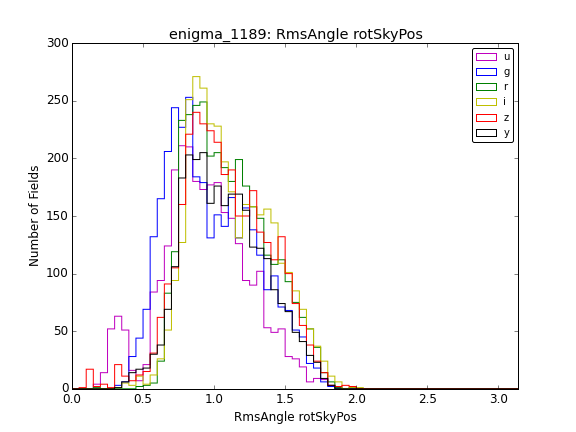
\includegraphics[width=\linewidth]{figs/enigma1189RmsAnglerotSkyPosugrizybandallpropsOPSIComboHistogram.png}
% \caption{The relative angle of the detector plane with respect to the sky, RotSkyPos, as a histogram showing the number of fields vs. rms of the parameter.}
% \label{RotSkyPos}
% \end{figure}

% The distribution of rms values by filter is shown in
% \autoref{RotSkyPos} for the current candidate baseline simulation,
% enigma\_1189.  As shown, the rms values cluster around the value 1
% radian,  with typical values 1 +- 0.3 radian.  This compares to a
% completely uniform distribution over the half circle with an rms of
% 1.14.  As mentioned above, uniformity in cosine squared is the goal.
% Simulated observing of 100 visits to a field show this will produce
% a factor of 10 decrease in CCD-based shear systematics such as edge
% effects and the brighter-fatter x-y anisotropy.




\newcommand\plottwo[2]{{%
\typeout{Plottwo included the files #1 #2}
\centering
\leavevmode
\includegraphics*[width=0.45\columnwidth]{#1}%
\hfil
\includegraphics*[width=0.45\columnwidth]{#2}%
}}%


%  rotSkyPos metrics

\begin{figure}[tbh!]
\plottwo{figs/WL/minion_1016_AngularSpread_rotSkyPos_propID_54_and_i_HEAL_SkyMap.pdf}
        {figs/WL/minion_1016_AngularSpread_rotSkyPos_u_g_r_i_z_y_propID_54_HEAL_ComboHistogram.pdf}
\caption{\textbf{Left:} Sky map showing the distribution of the AngularSpread
    metric applied to the angle $2 \times$ rotSkyPos, where rotSkyPos is the
    angle between the $+y$ camera direction and North, and the factor of two
    takes into account the degeneracy of angles separated by $\pi$ radians for
    spin-2 shear systematics.  An AngularSpread of 0 indicates a maximally
    anisotropic distribution (all visits have the same angle), while an
    AngularSpread of 1 indicates that visits are maximally balanced (the mean of
    $\cos \theta$ and $\sin \theta$ are both 0.) For the complete definition of
    the AngularSpread metric, please see the text.  To leading order, shear
    systematics permanently imprinted on the camera cancel when AngularSpread =
    1.  \textbf{Right:} Distribution of the AngularSpread metric applied to
    $2 \times$ rotSkyPos for all LSST filters.}
\label{fig:WL_AngularSpread_rotSkyPos}
\end{figure}

\begin{figure}[tbh!]
\plottwo{figs/WL/minion_1016_Kuiper_rotSkyPos_propID_54_and_i_HEAL_SkyMap.pdf}
        {figs/WL/minion_1016_Kuiper_rotSkyPos_u_g_r_i_z_y_propID_54_HEAL_ComboHistogram.pdf}
\caption{\textbf{Left:} Sky map showing the distribution of the Kuiper metric
    (see text for definition) applied to the angle rotSkyPos mod $\pi$.  A
    Kuiper value of 0 indicates an isotropic distribution of angles (mod $\pi$),
    while a Kuiper value of 1 indicates a maximally anisotropic distribution.
    \textbf{Right:} Distribution of the Kuiper metric applied to (rotSkyPos mod
    $\pi$) for all LSST filters.}
\label{fig:WL_Kuiper_rotSkyPos}
\end{figure}

%  ParallacticAngle metrics

\begin{figure}[tbh!]
\plottwo{figs/WL/minion_1016_AngularSpread_ParallacticAngle_propID_54_and_i_HEAL_SkyMap.pdf}
        {figs/WL/minion_1016_AngularSpread_ParallacticAngle_u_g_r_i_z_y_propID_54_HEAL_ComboHistogram.pdf}
\caption{Same as Fig. \ref{fig:WL_AngularSpread_rotSkyPos}, but for the
    parallactic angle (the angle between North and zenith) instead of rotSkyPos.
    The isotropy of the parallactic angle affects the impact of shear
    systematics due to telescope aberrations and differential chromatic
    refraction.}
\label{fig:WL_AngularSpread_ParallacticAngle}
\end{figure}

\begin{figure}[tbh!]
\plottwo{figs/WL/minion_1016_Kuiper_ParallacticAngle_propID_54_and_i_HEAL_SkyMap.pdf}
        {figs/WL/minion_1016_Kuiper_ParallacticAngle_u_g_r_i_z_y_propID_54_HEAL_ComboHistogram.pdf}
\caption{Same as Fig. \ref{fig:WL_Kuiper_rotSkyPos}, but for the parallactic
    angle instead of rotSkyPos.}
\label{fig:WL_Kuiper_ParallacticAngle}
\end{figure}


\subsection{Discussion}

The RotSkyPos metrics show that the majority of fields have good randomization
of detector angles projected on the sky.  The randomization of parallactic
angles is less successful, though this is to be expected due to fewer knobs
available to adjust the parallactic angle of observations of a given field.  In
both cases, however, a significant fraction of fields show metric values lower
than expected for a uniform distribution.  Regardless of the {\emph per field}
criterion adopted, it is desirable to avoid the incidence of individual
discrepant fields.  The recommended criterion for randomization of RotSkyPos and
parallactic angle is not the behavior of the majority of the fields, but of the
minority with the least random behavior -- the number of non-random fields
should be minimized.

It is certain that actively controlling the statistics of RotSkyPos will require
additional slewing of the camera rotator.  At present, the operations plan is to
only slew (beyond that required to track the sky during exposures) when
necessary to prepare for a filter change - that could be estimated at the
equivalent of $\simeq 3$ complete rotations per night.  To engage the rotator by
up to $\simeq 30$ degrees per visit would require $\simeq 300$ complete
rotations per night, though it may be possible to increase isotropy with far
less additional slewing.  The impact on survey efficiency and hardware wear and
tear has not been considered.  Whether or not this uniformity could be achieved
with less slew time if implemented in scheduling remains to be demonstrated.

Increasing the isotropy of the parallactic angle is trickier, since the
parallactic angle is only affected by the hour angle of observations (for a
given field).  It may be possible, however, to adjust the scheduler cost
function to better favor parallactic angle isotropy.


% The RotSkyPos metric analysis shows that the majority of fields have a
% good randomization of detector angles projected on the sky.
%
% There are some limitations to this observation.
%
% %First, we do not have at present a quantitative requirement for
% %randomization of this parameter.  In future development of weak
% %lensing analysis, a criterion should be developed.
%
% A significant fraction of fields  have median values that are
% lower or higher than expected for a random distribution, with some far
% from uniformly distributed.  Regardless of the $per field$ criterion,
% it is desirable to avoid the incidence of individual discrepant
% fields.
%
% The recommended criterion for randomization of RotSkyPos is not the
% behavior of the majority of the fields, but of the minority with the
% least random behavior.  The number of non-random fields should be
% minimized.  A recommended metric is the count of fields with median
% RMS less then 0.8 or greater than 1.5 radians (these values to be
% reviewed again as additional experience is gained with additional
% OpSim schedule simulations and weak lensing analysis.)
%
% It is certain that actively controlling the statistics of RotSkyPos
% will require additional slewing of the camera rotator.  At present,
% the operations plan is to only slew when necessary to prepare for a
% filter change - that could be estimated at the equivalent of $\simeq
% 3$ complete rotations per day.  \autoref{RotSkyPos} shows that to
% render the distribution completely uniform would require moving all
% observing angles an average of $\simeq 30$ degrees, or 300 complete
% rotations per night.  The timing of this has not been considered.
% Whether or not this uniformity could be achieved with less slew time
% if implemented in scheduling remains to be demonstrated.
%
% A similar metric for RotTelPos should be developed.


% --------------------------------------------------------------------

% ====================================================================
%+
% SECTION NAME:
%    photoz.tex
%
% CHAPTER:
%    cosmology.tex
%
% ELEVATOR PITCH:
%    Photometric redshifts are an intermediate data product that comprises
%    a key input for many investigations of galaxies and cosmology.  They
%    represent "static science", but we need them to have high quality after
%    the first year and at each "data release" thereafter.
%
% COMMENTS:
%    Updated Wed May 18 by MLG.
%    Minor updates to figures and captions, Sep 14 by MLG.
%
% BUGS:
%
%
% AUTHORS:
%   Melissa Graham, Sam Schmidt, Andy Connolly, Zeljko Ivezic
%-
% ====================================================================
\clearpage
\section{Photometric Redshifts}
\def\secname{photoz}\label{sec:\secname}

\credit{MelissaGraham},
\credit{SamSchmidt},
\credit{connolly},
\credit{ivezic}

\subsection{Introduction}

Photometric redshifts are an essential part of
every cosmology probe within LSST.  The principal concern for LSST
photo-$z$ performance is to meet the stringent requirements on redshift
uncertainty, bias, and catastrophic outlier rate as laid out in the
Science Requirements document. Photo-$z$'s are dependent on precise
measurements of galaxy colors, thus cadence and depth variations must be
examined as a function of all six LSST filter bandpasses.  Overall image
depth and signal-to-noise is our primary concern. For studies of Large
Scale Structure, Weak Lensing, Clusters, and Supernova host galaxies,
survey uniformity is desired for the full depth survey, while the
temporal details of how we reach full depth are not as important as
uniformity both as a function of sky position and observing conditions.
However, as we desire science-grade photometric redshifts after one year
of operations, two years, and so forth, the cadence must meet some basic
requirements for the six-band system at least on the timescales of the
yearly data releases.


\textbf{Specifications.} The Science Requirements Document (SRD) defines
the minimum statistical specifications for photometric redshifts for an
$i<25$, magnitude-limited sample of $4\times10^9$ galaxies from
$0.3<z<3.0$ as: (1) the root-mean-square ($\sigma$) error in photo-$z$,
divided by $1+z$, must be $\sigma < 0.02$; (2) the fraction of
``catastrophic" outliers (defined as those with errors exceeding the
larger of 0.06 or 3$\sigma$) must be $<10\%$; and (3) the average bias
must be $\overline{z_{\rm true} - z_{\rm phot}} < 0.003$. With this in
mind, we are developing software to show that our photo-$z$ algorithms
can meet specifications for LSST baseline parameters and to simulate the
impact of deviations from the 10-year baseline plan on photo-$z$
statistics.

\textbf{Planned Experiments.} This software is designed to allow the
user to modify LSST baseline parameters, simulate a set of test galaxy
observations (i.e., magnitudes with errors appropriate for the given
LSST parameters) from a training catalog with ``true" magnitudes and
redshifts and a realistic intrinsic dispersion in color, magnitude, and
redshift, run a photometric redshift algorithm on the test galaxies
(i.e., matching in color-space to the training catalog), and output
statistics for analysis. Modifiable LSST input parameters will include:
the limiting magnitude applied to the galaxy catalogs (e.g., $i<25$);
the number of visits per filter; the number of years of LSST
observations that have passed (this can be a fraction of a year);
systematic offsets to the magnitudes in each filter (default $=0$); and
coefficients for the magnitude uncertainties in each filter (default
$=1$).  Output for user analysis will include catalogs of $z_{\rm true}$
$vs.$ $z_{\rm phot}$ and the aforementioned statistics on the photo-$z$
in any desired redshift range. For example, we will be able to vary the
total number of $u$-band visits and examine how this affects the
fraction of outliers at 1, 5, and 10-years of the survey. In this
software, parameters of the photo-$z$ algorithm itself will also be
modifiable, allowing us to test options in the algorithms against
various LSST observing strategies.

\textbf{Currently implemented photo-$z$ algorithm.} We draw $N_{\rm
test}$ ``test" galaxies from the training catalog, determine their
magnitude uncertainties as appropriate for the LSST parameters, randomly
scatter their magnitudes to induce an observational error, and calculate
the associated colors and color errors. We calculate the Mahalanobis
distance in color space between each test galaxy and all training
catalog galaxies, and identify a color-matched subset using a threshold
defined by the $\chi^2$ percentage point function at 95\%. We draw a
random color-matched training galaxy and use its redshift as the
photo-$z$ for that test galaxy. We then calculate our statistical
metrics on the photometric redshifts for the test sample, using each
test galaxy's original catalog redshift as the ``true'' redshift. This
process is open to substituting alternate photometric redshift
algorithms, a variety of galaxy catalogs, and/or adding priors based on
e.g., apparent magnitude.


\subsection{Metrics}

The primary metrics we will use to evaluate LSST
observing strategies with respect to the SRD photo-z specifications are the
standard deviation, bias, and fraction of outliers. For all test
galaxies we calculate $\Delta z = (z_{\rm true} - z_{\rm phot}) /
(1+z_{\rm true})$, and identify galaxies in the interquartile range of
$\Delta z$. For these interquartile galaxies we determine the standard
deviation, $\sigma$, of the $\Delta z$ distribution, and the bias as the
median value of $\Delta z$. The interquartile range is used to exclude
outliers from influencing these statistics; in other words, they
represent the standard deviation and bias for the subset of ``good"
photo-$z$'s. The ``catastrophic" outliers are identified as those with
$\Delta z$ exceeding the larger of 0.06 or 3$\sigma$.


\subsection{Initial Results}

To demonstrate this software with a
preliminary analysis, we apply the currently implemented photo-$z$
algorithm to a catalog of galaxies that was originally created as an
accurate cosmological simulation for Euclid. We first cull the catalog
to galaxies with $i$-band magnitude $<25.3$, and then randomly draw
training and test galaxy samples (with at least a 4$\times$ more
galaxies in the training sample than the test sample). For this
demonstration we show how the photo-$z$ metrics evolve with respect to
two of the basic LSST parameters: the year of the survey, and the number
of $u$-band visits. When we simulate results in a given year of LSST, we
assume uniform progression in all filters (i.e., the total number of
visits per filter, \texttt{[56, 80, 184, 184, 160, 160]} in
\texttt{[u,g,r,i,z,y]}, is distributed evenly over all years). When we
simulate the LSST 10-year results for a given number of $u$-band visits,
the visits removed/added to $u$-band are added/subtracted evenly to/from
the other five filters. The results of these tests are presented in
Figure~\ref{fig:redshifts} and~\ref{fig:metrics}. For example, in this
demonstration we can see that the $u$-band is necessary to limit scatter
at $z<0.5$ and $z>2.0$.

\begin{figure}[h]
\begin{center}
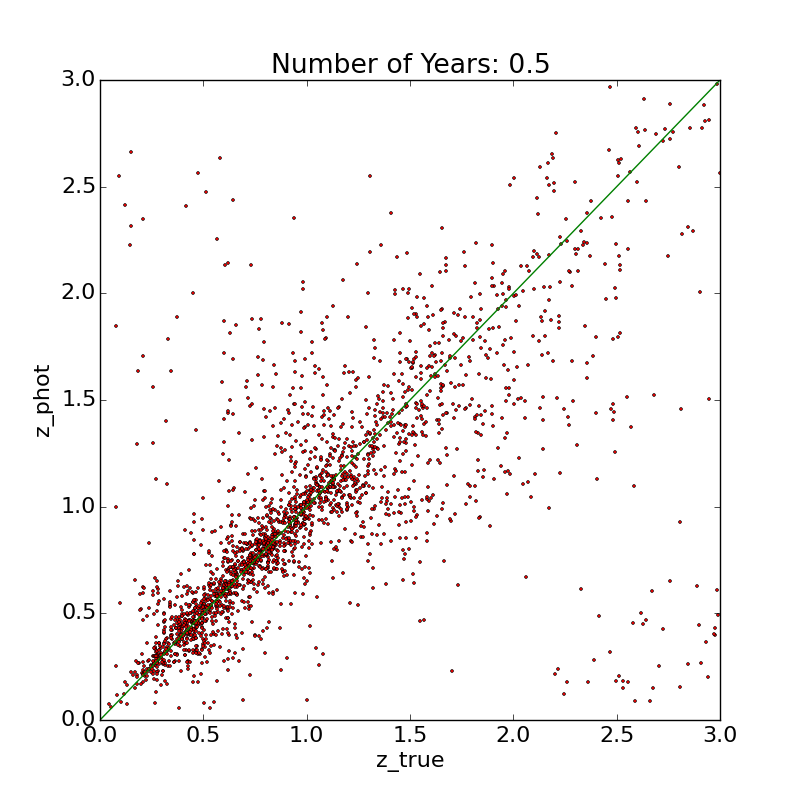
\includegraphics[width=5cm]{figs/photoz/nyears_cat05.png}
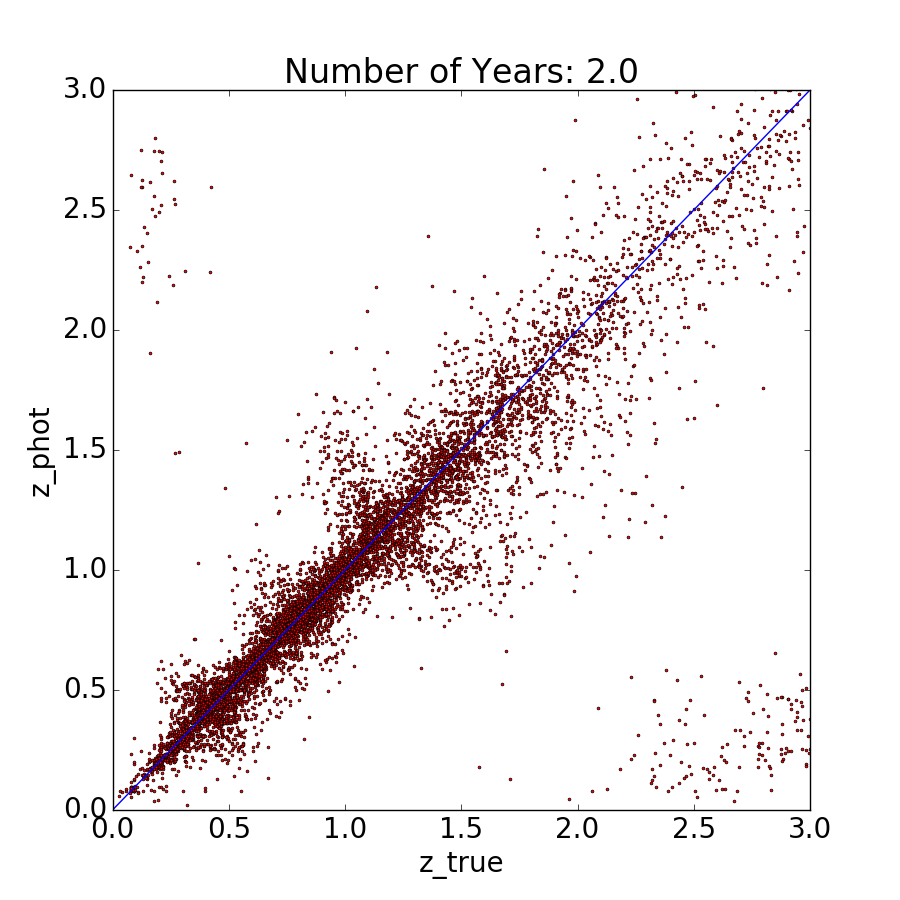
\includegraphics[width=5cm]{figs/photoz/nyears_cat20.png}
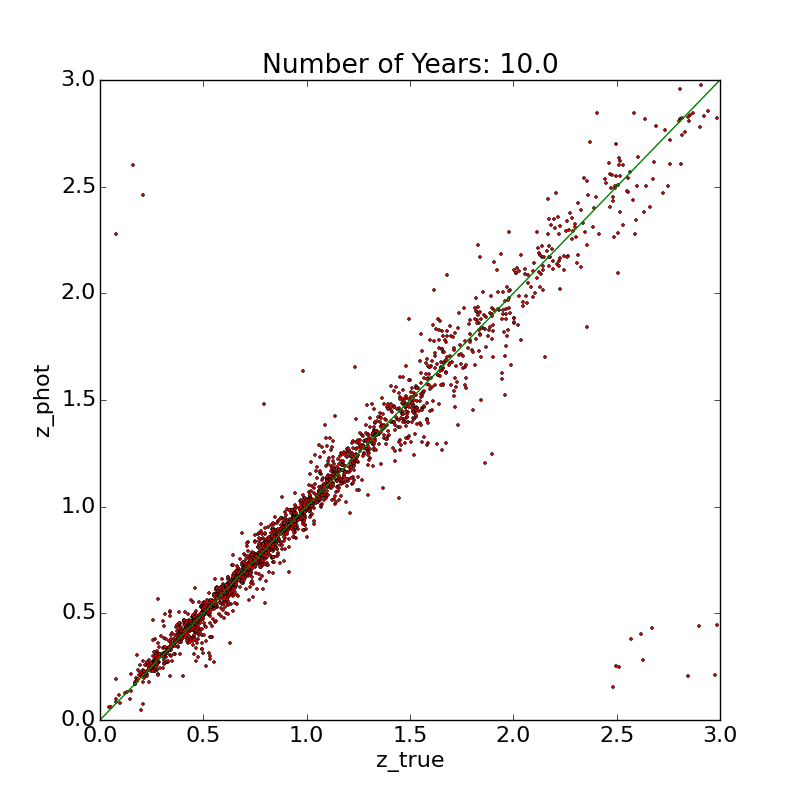
\includegraphics[width=5cm]{figs/photoz/nyears_cat100.png}
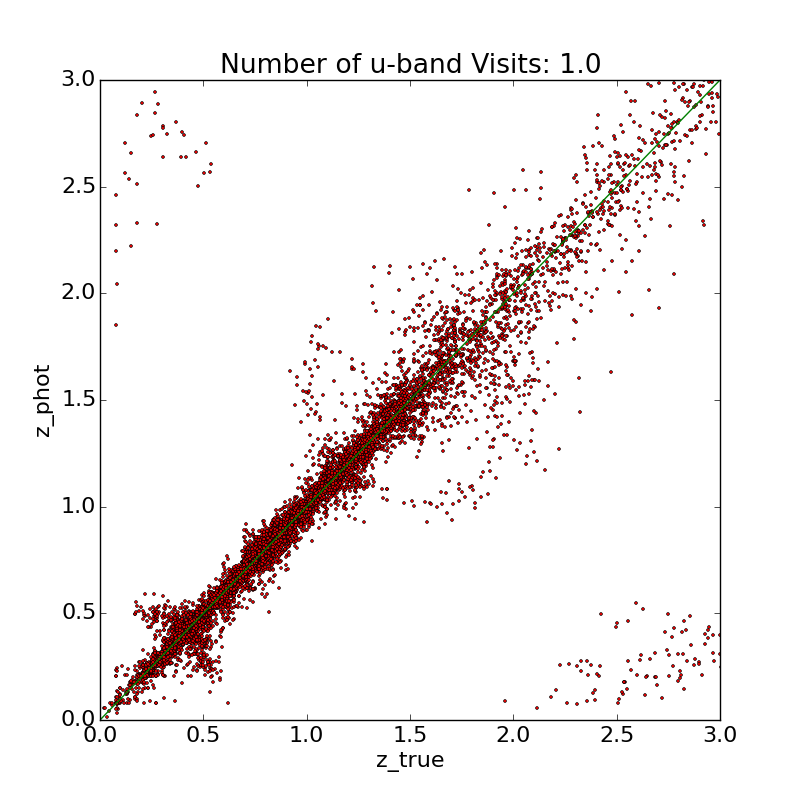
\includegraphics[width=5cm]{figs/photoz/uvisits_cat1.png}
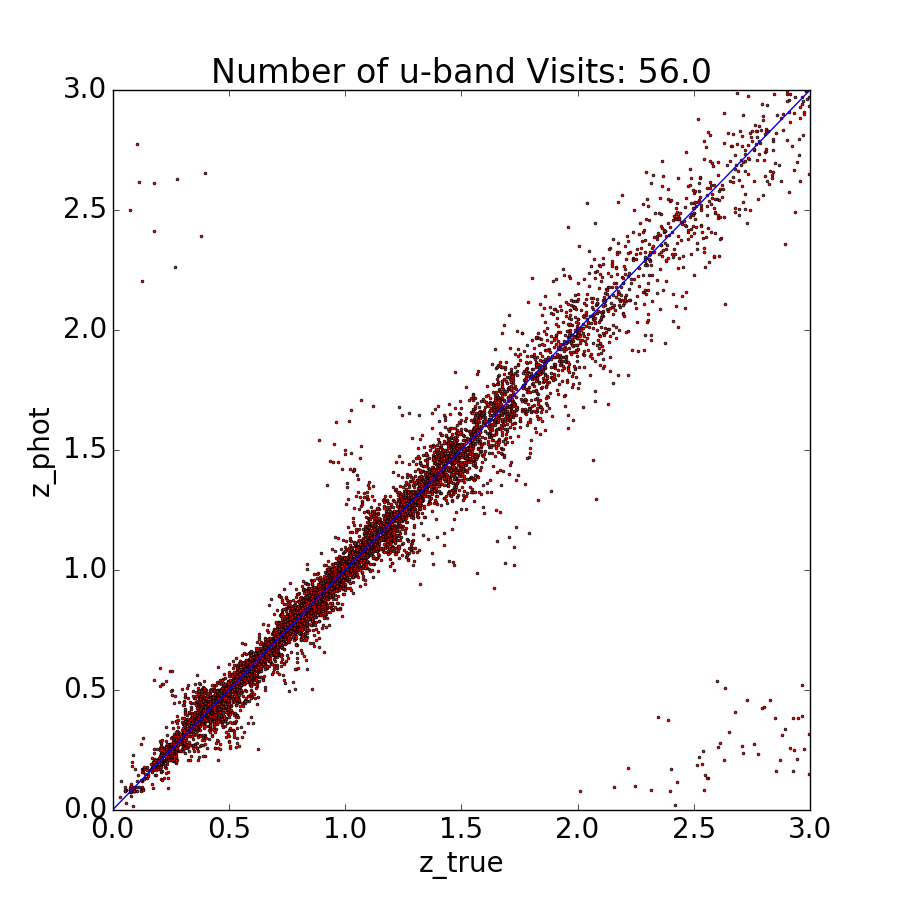
\includegraphics[width=5cm]{figs/photoz/uvisits_cat4.png}
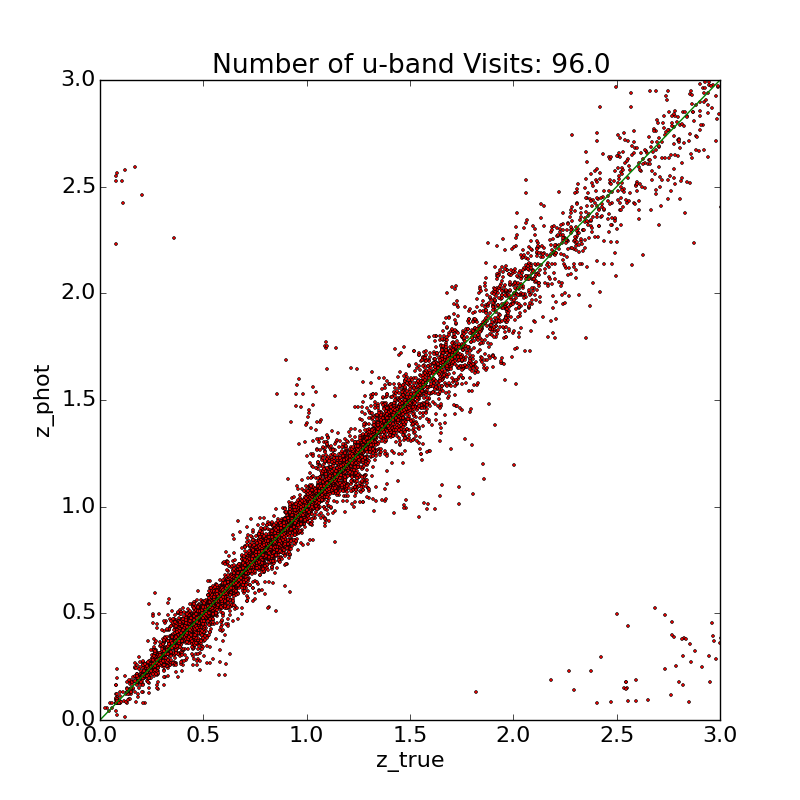
\includegraphics[width=5cm]{figs/photoz/uvisits_cat6.png}
\caption{Photometric vs. spectroscopic (i.e., catalog truth) redshifts
for our preliminary simulations. Across the top row we show results from
0.5, 2.0 and 10.0 years of the LSST survey using catalogs with 10000 test
and 40000 training galaxies. The photo-$z$'s clearly improve with time
as the survey progresses. Across the bottom row we show results for $1$,
$56$ (baseline), and $96$ $u$-band visits, also using catalogs with 10000 test
and 40000 training galaxies. Between the left-most and middle plot of
the bottom row, representing 1 and 56 (baseline) $u$-band visits
respectively, we see that $u$-band data is necessary to limit scatter in
the photo-$z$'s, especially at $z<0.5$ and $z>2.0$.
\label{fig:redshifts}}
\end{center}
\end{figure}

\begin{figure}[h]
\begin{center}
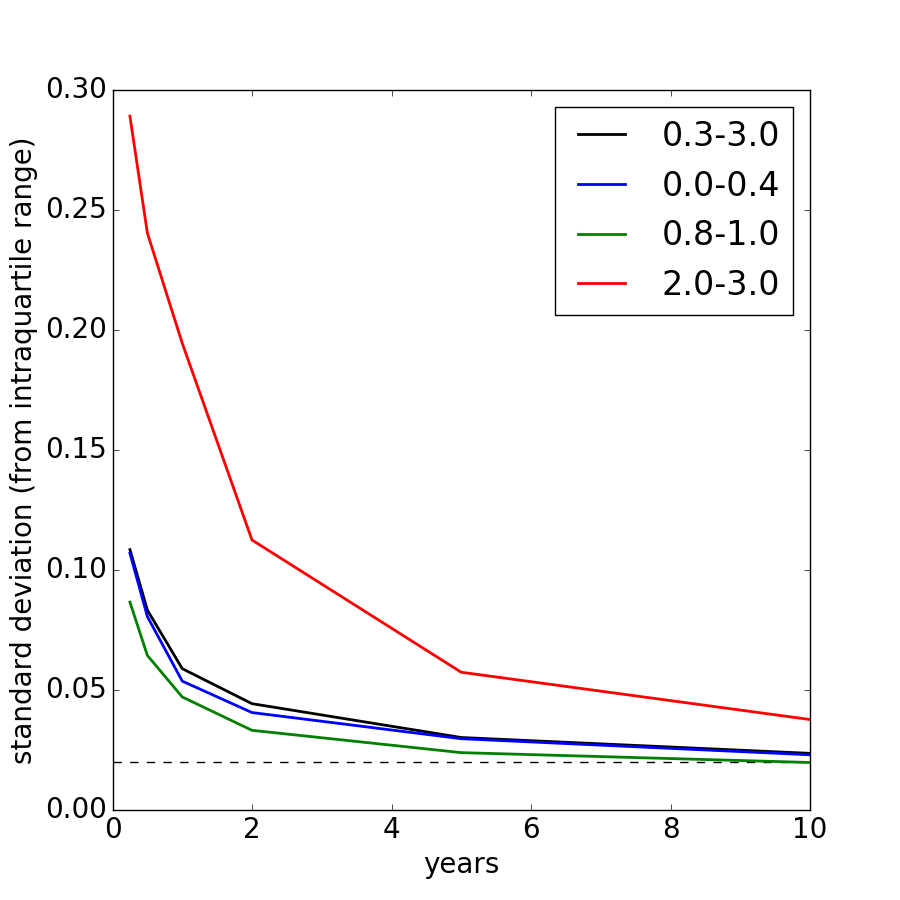
\includegraphics[width=5cm]{figs/photoz/nyears_IQR.png}
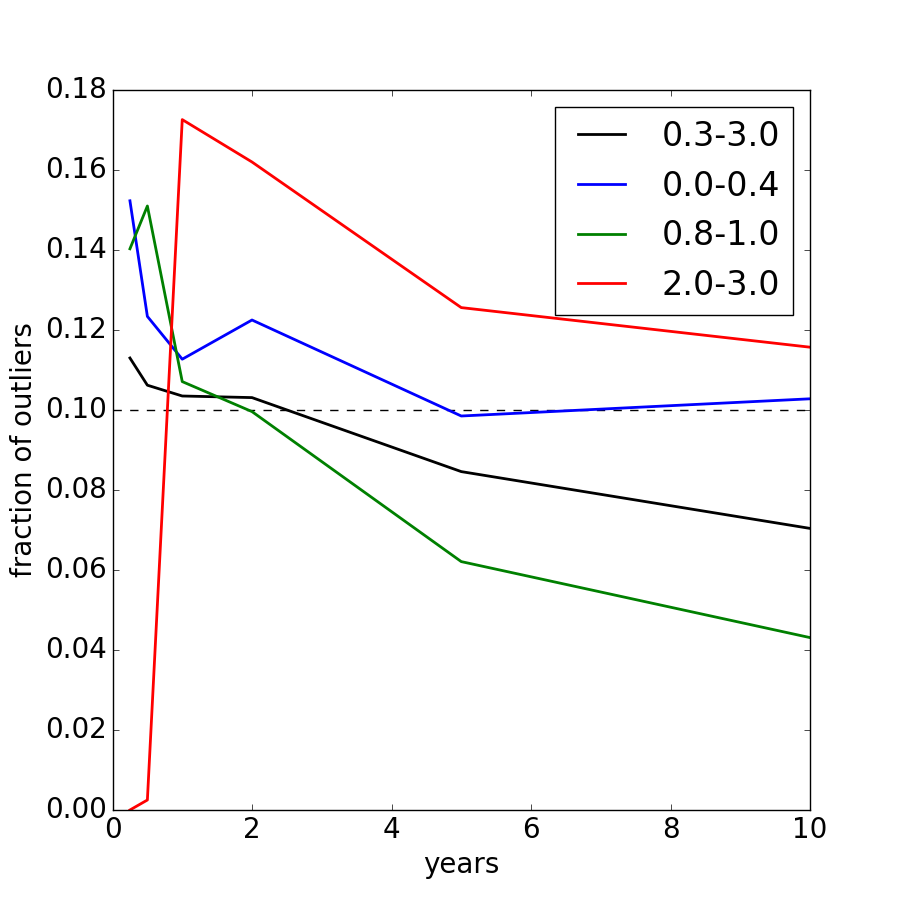
\includegraphics[width=5cm]{figs/photoz/nyears_fout.png}
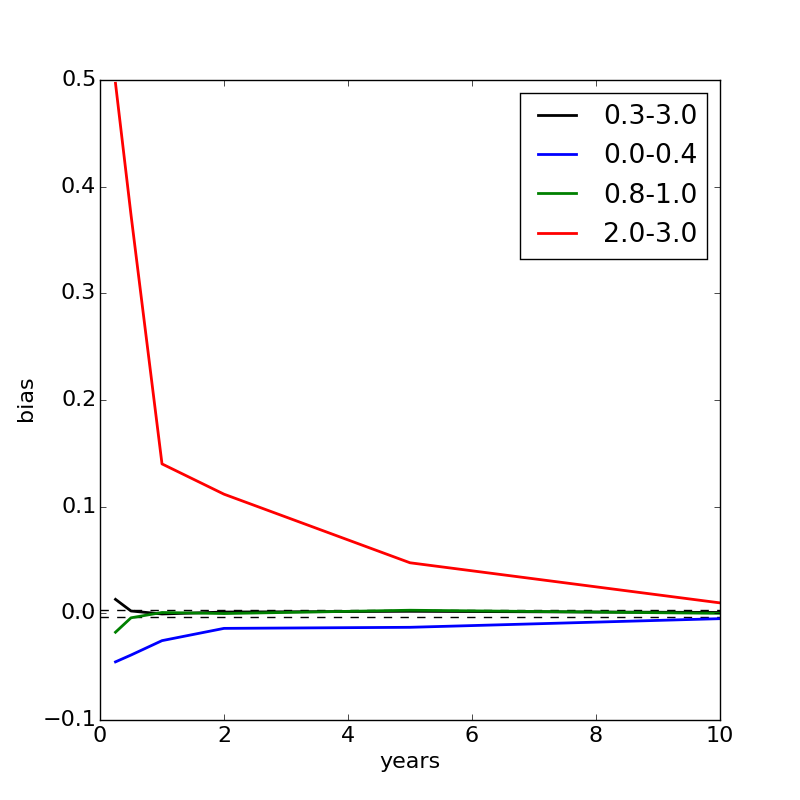
\includegraphics[width=5cm]{figs/photoz/nyears_bias.png}
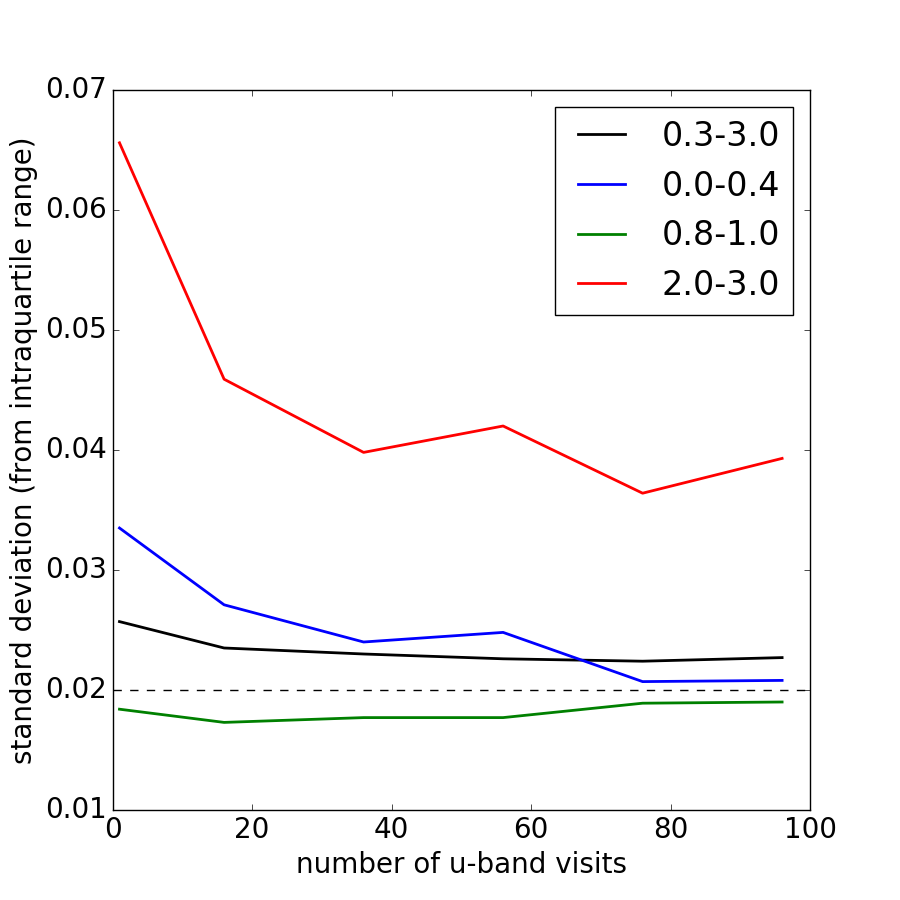
\includegraphics[width=5cm]{figs/photoz/uvisits_IQR.png}
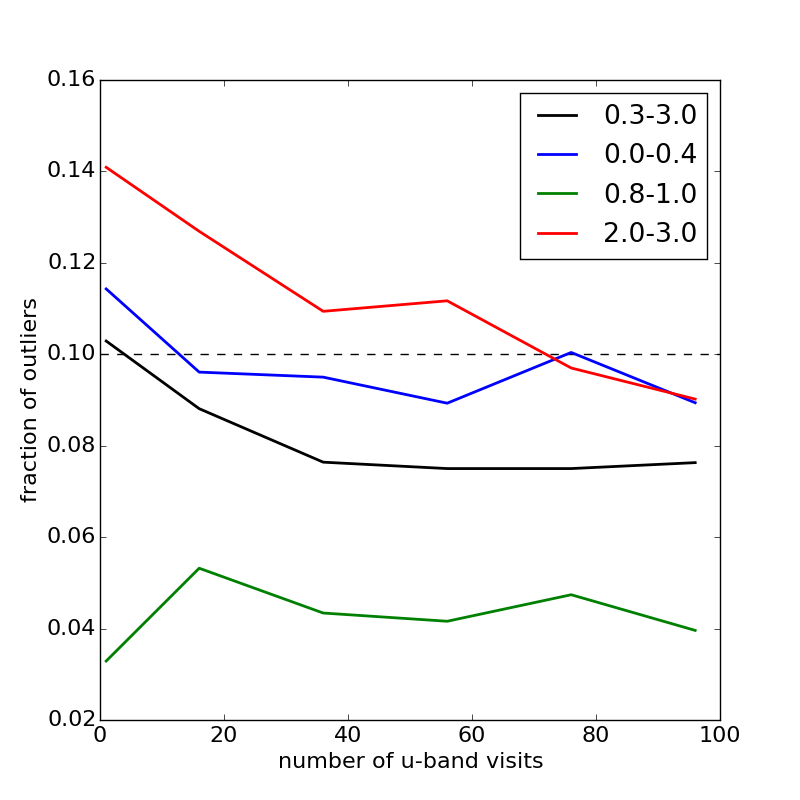
\includegraphics[width=5cm]{figs/photoz/uvisits_fout.png}
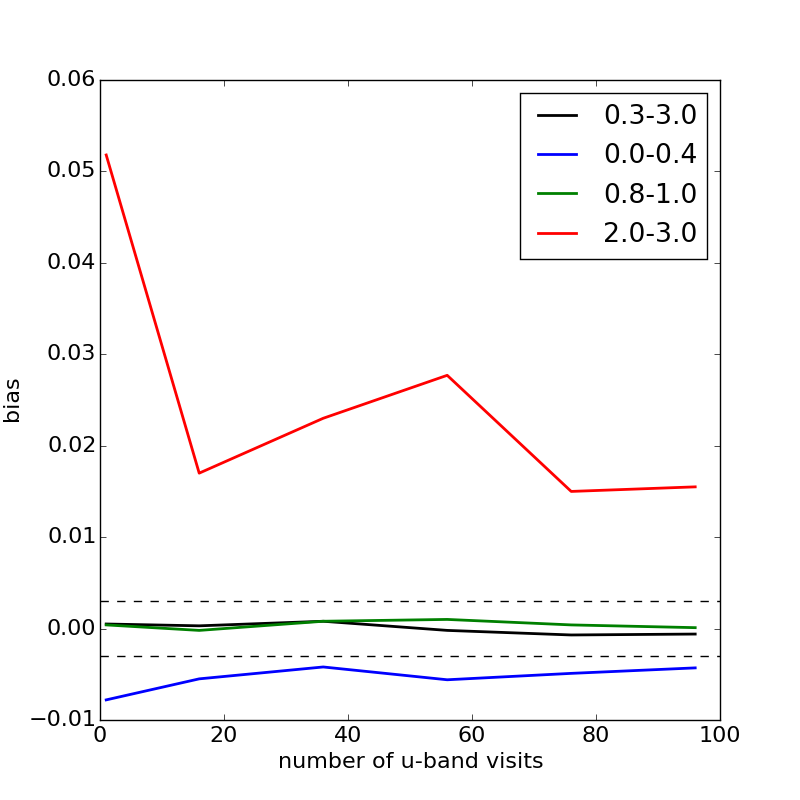
\includegraphics[width=5cm]{figs/photoz/uvisits_bias.png}
\caption{Three photo-$z$ metrics as a function of LSST parameters. From
left to right, the y-axis is the standard deviation, the fraction of
outliers, and the bias. The top row shows these statistics as a function
of the number of years of LSST survey, and the bottom row shows them as
a function of the number of $u$-band visits. Colors show these relations
for four bins in redshift: 0.3--3.0 (black), 0.0--0.4 (blue), 0.8--1.0
(green), and 2.0--3.0 (red). Dashed lines mark the SRD specification for
each metric. The fraction of catastrophic outliers appears erroneously
low early in the LSST survey (top middle plot) when the dispersion in
$z_{\rm spec}-z_{\rm phot}$ is too large to adequately identify outliers
(e.g., see top left plot of Figure \ref{fig:redshifts}).
\label{fig:metrics}}
\end{center}
\end{figure}


\subsection{Discussion}

\textbf{Additional considerations for observing strategy.} As mentioned
above, overall image depth and signal-to-noise is our primary concern,
so we are not testing changes in e.g., the inter-night gap time or the
exposure time of individual visits.  Our software is instead focused on
modifying other LSST parameters such as systematic offsets to the
magnitudes in each filter and/or coefficients for the magnitude
uncertainties in each filter in order to simulate improvements or
degradations the system throughput, sky background brightness, and other
such factors. We also aim to test airmass distributions (i.e., changes
to the effective filter functions), different progression rates for
filters (e.g., a scenario in which we complete all $u$-band by year 2),
scenarios in which some areas of sky have better/worse coverage at any
given time, and so forth. In all respects we are open to suggestions
from the community.

\textbf{Considerations for building the real training catalog.} All
photometric redshift algorithms require training set data consisting of
objects with secure spectroscopic redshifts.  For LSST, many of these
will be contained in a small number of training/calibration fields (e.g.
COSMOS, VVDS).  Imaging these fields to full depth in all six bands
early in the survey (but under the range of observing conditions
expected for the ten year survey) will be key to characterizing
performance.  Inclusion of these patches of full-depth imaging must be
included in any cadence design. Future simulations of photo-$z$ results
can include varying the quality of the training catalog obtained by
LSST.

\textbf{Integration with MAF.} One way to extend our program to be able
to evaluate observing strategies simulated with \OpSim could be to use
the MAF to enable us to simulate representative samples of galaxies
across the mock LSST sky, and compute the metrics we have defined.
It may be possible to avoid such a large computation by first defining
some intermediate diagnostic metrics, such as the $u$-band coverage, and
working out how our higher level metrics depend on them, using some
approximate interpolation formulae.

\textbf{Connecting to the Dark Energy Figure of Merit.} The metrics we
have defined here should be able to be related to the DETF Figure of
Merit, but because photo-zs affect all of the LSS, WL and CL
cosmological probes, this step may need to wait until a joint
Figure of Merit MAF metric is developed.

% --------------------------------------------------------------------
%
% \subsection{Conclusions}
%
% Here we answer the ten questions posed in
% \autoref{sec:intro:evaluation:caseConclusions}:
%
% \begin{description}
%
% \item[Q1:] {\it Does the science case place any constraints on the
% tradeoff between the sky coverage and coadded depth? For example, should
% the sky coverage be maximized (to $\sim$30,000 deg$^2$, as e.g., in
% Pan-STARRS) or the number of detected galaxies (the current baseline but
% with 18,000 deg$^2$)?}
%
% \item[A1:] ...
%
% \item[Q2:] {\it Does the science case place any constraints on the
% tradeoff between uniformity of sampling and frequency of  sampling? For
% example, a rolling cadence can provide enhanced sample rates over a part
% of the survey or the entire survey for a designated time at the cost of
% reduced sample rate the rest of the time (while maintaining the nominal
% total visit counts).}
%
% \item[A2:] ...
%
% \item[Q3:] {\it Does the science case place any constraints on the
% tradeoff between the single-visit depth and the number of visits
% (especially in the $u$-band where longer exposures would minimize the
% impact of the readout noise)?}
%
% \item[A3:] ...
%
% \item[Q4:] {\it Does the science case place any constraints on the
% Galactic plane coverage (spatial coverage, temporal sampling, visits per
% band)?}
%
% \item[A4:] ...
%
% \item[Q5:] {\it Does the science case place any constraints on the
% fraction of observing time allocated to each band?}
%
% \item[A5:] ...
%
% \item[Q6:] {\it Does the science case place any constraints on the
% cadence for deep drilling fields?}
%
% \item[A6:] ...
%
% \item[Q7:] {\it Assuming two visits per night, would the science case
% benefit if they are obtained in the same band or not?}
%
% \item[A7:] ...
%
% \item[Q8:] {\it Will the case science benefit from a special cadence
% prescription during commissioning or early in the survey, such as:
% acquiring a full 10-year count of visits for a small area (either in all
% the bands or in a  selected set); a greatly enhanced cadence for a small
% area?}
%
% \item[A8:] ...
%
% \item[Q9:] {\it Does the science case place any constraints on the
% sampling of observing conditions (e.g., seeing, dark sky, airmass),
% possibly as a function of band, etc.?}
%
% \item[A9:] ...
%
% \item[Q10:] {\it Does the case have science drivers that would require
% real-time exposure time optimization to obtain nearly constant
% single-visit limiting depth?}
%
% \item[A10:] ...
%
% \end{description}


\navigationbar

% ====================================================================


% --------------------------------------------------------------------

% ====================================================================
%+
% SECTION:
%    supernovacosmology.tex
%
% CHAPTER:
%    cosmology.tex
%
% ELEVATOR PITCH:
%    SNIa cosmology, approach to evaluating dependence of science on cadence
%
% COMMENTS:
%
%
% BUGS:
%
%
% AUTHORS:
%    Phil Marshall (@drphilmarshall)  - put your name and GitHub username here!
%-
% ====================================================================

\section{Supernova Cosmology and Physics}
\def\secname{supernovae}\label{sec:\secname}
% \label{sec:cosmology, supernovae, classification, lenstimedelays, deepdrillingfields }

\noindent{\it Jeonghee Rho, Michelle Lochner, Rahul Biswas, Seth Digel} % (Writing team)

% This individual section will need to describe the particular
% discoveries and measurements that are being targeted in this section's
% science case. It will be helpful to think of a ``science case" as a
% ``science project" that the authors {\it actually plan to do}. Then,
% the sections can follow the tried and tested format of an observing
% proposal: a brief description of the investigation, with references,
% followed by a technical feasibility piece. This latter part will need
% to be quantified using the MAF framework, via a set of metrics that
% need to be computed for any given observing strategy to quantify its
% impact on the described science case. Ideally, these metrics would be
% combined in a well-motivated figure of merit. The section can conclude
% with a discussion of any risks that have been identified, and how
% these could be mitigated.

This section is concerned with the detection and characterization of supernovae (SNe)
over time with LSST and their various scientific applications.
The most important
application is the use of supernovae type Ia (SNIa) and potentially some core-collapse SN (like type IIP) to trace the recent expansion history of the universe,
and confront models of the physics driving the late time accelerated expansion
of the universe. 

This objective of SN cosmology follows (at least for SNIa) results from several
highly successful surveys; improvement in knowledge of cosmology could come from
substantially larger numbers of well-characterized SNe.
This
goal is not directly tied to the unprecedentedly large survey area of LSST.  
However, we shall argue that in practice, even this
goal would benefit from the spatial scale offered by the WFD
component of the LSST survey. 

On the other hand, the WFD aspect will make the LSST survey potentially the 
first to scan the very large area of the entire Southern sky for SNe. 
SNe that are detected and well characterized by LSST will
probe the isotropy of the universe.  Peculiar velocities of 
SNe will probe the growth of structure.  In addition, this large sample
will enable further
sharpening of our understanding of the properties of the SN population 
of different types. 
This last point is extremely important for SN cosmology goals:  The success of SNIa cosmology has always been based on the empirical model that intrinsic peak brightnesses are related to the certain observable characteristics of SNe. 
%While the spatial locations of the SNe are not important
The 
WFD SNIa sample will dramatically increase the size of the sample 
available to train such an empirical model, as well understand the probability of deviations and scatter from this model. Aside from issues like calibration 
which need to be addressed differently, a larger sample of such well measured SNe is probably the only way to address `systematics' due to deviations from the empirical
model. The anticipated sample can be thought of as consisting of two 
components:  the low-redshift sample which is more likely to be complete, and the higher-redshift sample that will be able to constrain evolution. 
% --------------------------------------------------------------------

\subsection{Target measurements and discoveries}
\label{sec:keyword:targets}

% Describe the discoveries and measurements you want to make.

SNe of different types are visible over time scales of about a few 
weeks (e.g., type Ia) to nearly a year (type IIP).  During the full ten-year
 survey, LSST will scan the entire southern sky repeatedly
 with a WFD cadence, and certain specific locations
of the sky called the Deep Drilling Fields (DDF) with special enhanced cadence. 

This spatio-temporal window should contain millions \todo{RB}{remember to check} of SNe, that will have apparent magnitudes brighter than the single exposure limiting magnitude of LSST.  However, the actual
 sequence of observations by LSST, defined by the series of field pointings as a
 function of time in filter bands (along with weather conditions), will
 determine the extent to which each SN can be detected and
 characterized well.  Characterization of the SNe is at the core of a
 number of science programs that use them as bright, abundant objects with empirically determined intrinsic brightnesses. For LSST, this goal entails (a) detection of SNe, (b) photometric typing of SNe, (c) estimating photometric redshifts of SNe (or identifying host galaxies 
 and obtaining their redshifts from photometry or follow-up spectroscopy),
(d) estimation of intrinsic brightnesses of the SNe, and finally (e) use of these data in addressing our science goals of cosmological inference, etc.
The efficacy of photometric typing, redshifts and estimation of intrinsic brightnesses are all
dependent on the amount of information available in the observed light curves of SNe. While these steps are not necessarily independent, it is useful to think of the requirements on some of these steps separately; it is not unlikely  that combinations of some of the steps would still be affected by similar requirements. 

{\emph{Our first objective is to detect such SNe}}, by which we mean
selecting SNe from among the transient sources detected by LSST.
% classify them as SNe (as opposed to an AGN, or an asteroid). 
In brief, this process 
consists of defining a set of image subtractions between a high-resolution
`template` image of a sky section, and a set of single exposures at
different times (usually of lower resolution) of the same region, after 
accounting for the different resolutions of images, and alignments. These sets of image subtractions associated
 with a single object will be used to detect the object as a transient and then
classify the transient as an SN. Clearly, detecting an SN depends on the number of such images recorded per object, the different filters used for those images, and the signal-to-noise ratios of the images. %One might expect that 
The efficiency of this step may be summarized as a threshold on the joint properties 
of an astrophysical candidate (apparent brightness, light curve characteristics, background) as well as observing conditions (astronomical seeing, etc.).  

{\emph{Our second objective is to photometrically classify different kinds of SNe.}} 
%{\bfseries Photometric SN classification}\\
Previously, only spectroscopically typed SNe have been used for cosmology. Photometric 
typing from light curves alone has only been used to select candidates for spectroscopic 
follow-up (see, e.g., \citet{Sako2008}). However, LSST will simply find far too many 
candidates for even a significant fraction of them to be followed up spectroscopically. In order to avoid 
discarding the majority of the SN dataset, we need to use techniques capable of 
determining cosmological parameters from a potentially contaminated photometric SN dataset.

Several techniques have been proposed recently to solve this problem. One 
approach involves applying stringent cuts to the photometric dataset to obtain a nearly pure sample 
of SNIa\citep{Bernstein2012,Campbell2013} and running the standard SNIa cosmology analysis 
with this sample. Another approach, BEAMS \citep{Kunz2007,Newling2011,Hlozek2012,Knights2013}, 
makes use of an entire dataset, coping with contamination by using a mixture model for the 
likelihood, thus allowing for multiple populations. Whatever the technique ultimately used for 
cosmological analysis, it will rely on accurate initial classifications of SN type and 
unbiased estimates for the probability of each type.

Current state-of-the-art photometric classification techniques rely on fitting empirically 
determined templates of SNe to light curves \citep{Jha2007,Guy2007,Sako2011}. However in 
recent years, new approaches have been developed in response to the 2010 `Supernova 
Photometric Classification Challenge' \citep{Kessler2010a}. Many of these use novel light curve 
parameterization and employ machine learning algorithms to perform the classification (see \citet{Kessler2010b} and references therein).

While many of these methods have been tested on standard sets of simulated data and (in some cases) 
on SDSS data, which technique (if any) is superior in all situations is unclear. For 
example, some techniques are dependent on the availability of reliable redshift information. 
%, while others  are less reliant on it. 
Some techniques may be more robust to non-representative datasets [Not sure what this means] than 
others, and how the techniques will respond to changes in cadence, filter sets, signal-to-noise, 
etc., is unclear.  

With this in mind, we propose the use of a multifaceted classification system which employs 
several different methods for extracting features from the light curves (e.g., fitting parametric 
functions or templates) and several different classification algorithms. This system is highly 
modular, allowing new approaches for direct comparison with existing  techniques to be added easily. This also allows direct analysis of different observing strategies, without requiring 
an initial choice of classification technique. 


{\emph{Our third objective is to characterize SNe in terms of empirical
    light curve models.}}

The ultimate goal of using SNe (type SNIa or SNIIP) for cosmology requires estimating the intrinsic brightnesses of the SN. The
first (and sometimes only, depending on the light curve model) step is
fitting the calibrated fluxes to a light curve model with a set of parameters.
According to the ansatz used in SN cosmology, the intrinsic brightness of
 SNe is largely determined by the parameters of the light curve model; 
 hence the uncertainties on the inferred parameters largely determine the
 uncertainties on the inferred peak intrinsic brightness or distance moduli of the SNe.

% Now, describe their response to the observing strategy. Qualitatively,
% how will the science project be affected by the observing schedule and
% conditions? 

% In broad terms, how would we expect the observing strategy
% to be optimized for this science?





% --------------------------------------------------------------------

\subsection{Metrics}
\label{sec:keyword:metrics}

Quantifying the response via MAF metrics: definition of the metrics,
and any derived overall figure of merit.
\label{sec:keyword:metrics}

\begin{center}
\begin{tabular}{| p{5cm} |p{10cm} |p{2cm}}
\hline Metric & Description & Status\\
\hline
Discovery Metric &  Identify the number of LSST data points and quality required & \\
SN light curve quality & Generate SN light curves using OpSim output of baseline Cadence &\\
SN classification & Classify identified SNe into SN Ia, II, Ib, and Ic & \\
SN light curve II & Generate SN light curves with different redshift (0.1-1) &\\
SN discovery II &  Estimate the number of SN discovery as a function of redshift & \\
\hline \end{tabular}
 \end{center}

\subsubsection{Discovery Metric}
This metric is related to the estimated pr


\emph{To be added: discussion of the ROC curve as a useful metric for photometric supernova 
classification}


\begin{figure*}[!hb]
    \begin{minipage}[b]{\linewidth}
        \includegraphics[width=\textwidth]{figs/supernova/fig_firstSeason_0}
        \includegraphics[width=\textwidth]{figs/supernova/fig_firstSeason_1}
        \includegraphics[width=\textwidth]{figs/supernova/fig_firstSeason_2}
        \includegraphics[width=\textwidth]{figs/supernova/fig_firstSeason_3}
        \includegraphics[width=\textwidth]{figs/supernova/fig_firstSeason_4}
    \end{minipage}
\label{fig:opsimSummary}
\caption{Include 1) an example of Type Ia Light Curve, 2) an example of Type II, 3) the number of SNR as a function of
redshift}
\end{figure*}


% --------------------------------------------------------------------

\subsection{OpsSim Analysis}
\label{sec:keyword:analysis}

{\bf Motivation and description:}

As noted above the scientific goal of characterizing SNe is to a large extent
dependent on how well the light curves of individual SNe are sampled in
time and filters. To study this, we re-index the OpsSim output on spatial
locations rather than use the temporal index. There are different methods for this (which will be merged), and here we will first illustrate this in terms the cadence in an example LSST field.
Our goal for observing strategy is to obtain 7-10 epochs spread over 50 days or so for more than one filter (we will quantify the mininum filters later in the Section). This will increase the number of well-measured SNe at low redshift (z$<$ 1) and improve distinguishing SN Ia from other types of SNe.

{\bf Analysis Results and Discussion}
We analyzed the Opsim output of the baseline observing strategy (see Section 2.2),
$enigma\_1189\_sqlite.db$ {\footnote {\url{http://ops2.tuc.noao.edu/runs/}}}, and 
we made our analysis with two separate data sets, one with Deep Drilling fields and the other one with the main WFD survey.

\begin{figure}[tbh!]
%\vskip -1.3in
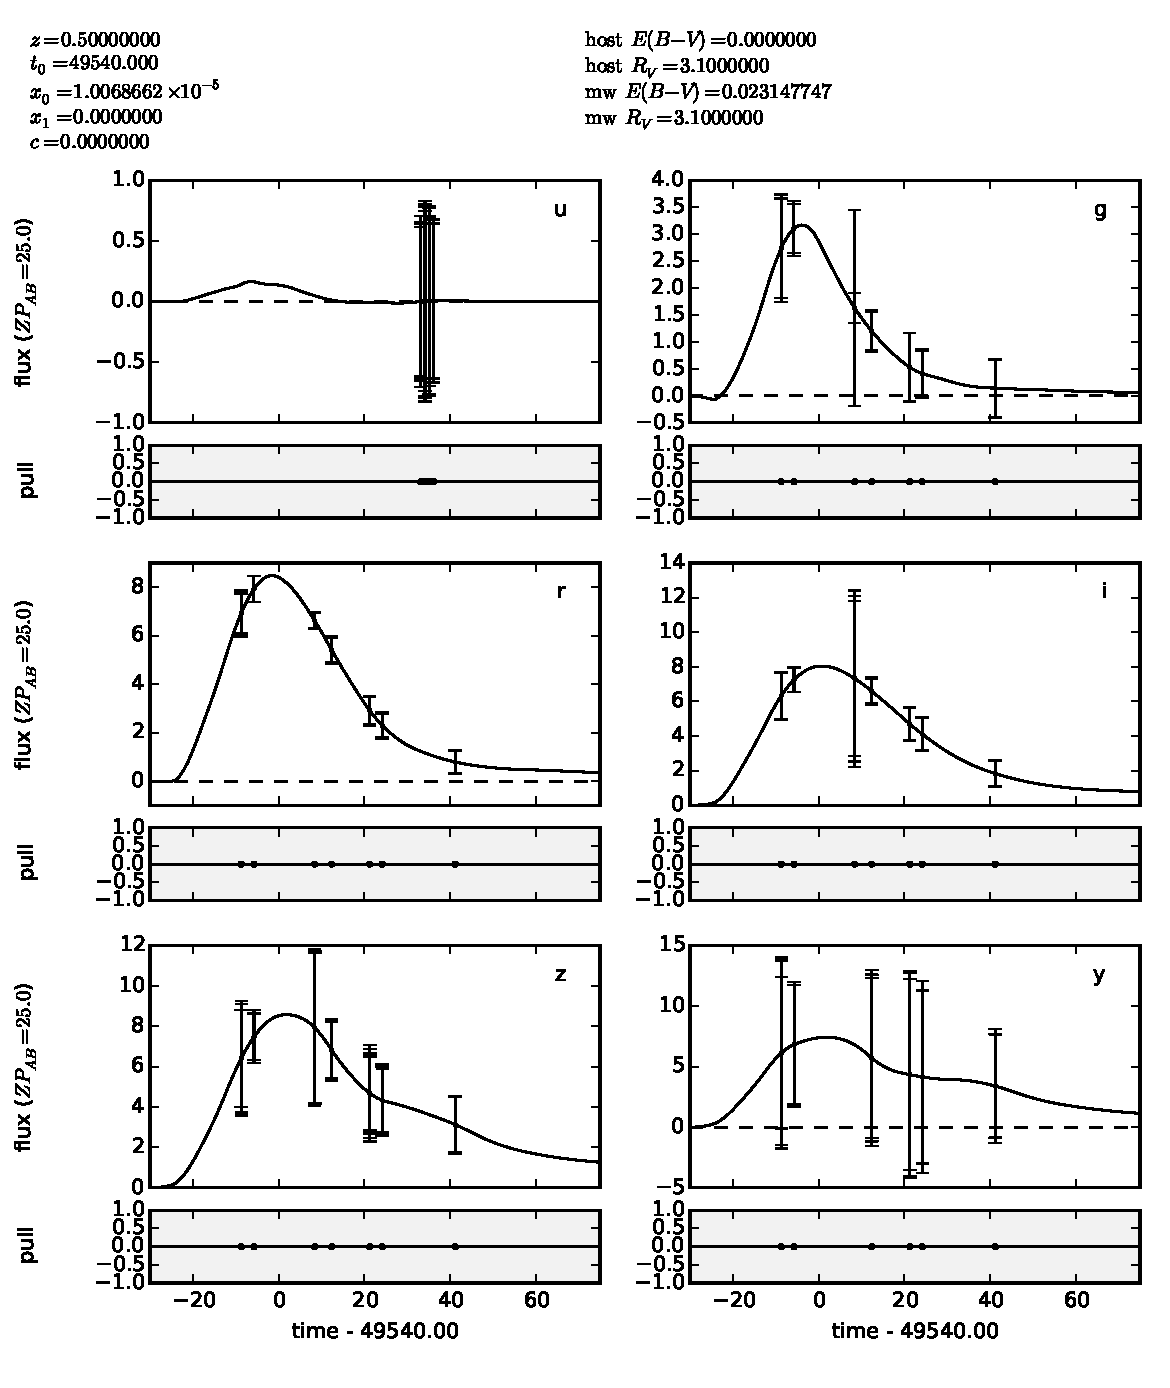
\includegraphics[angle=0,width=0.99\hsize:,clip]{figs/SN_290_lc.pdf}
%\vskip -1.3in
\caption{Light curves of Supernova Type Ia generated using Deep Drilling Survey of the OpSim output in 6 different bands.
}
\label{fig:SNIaLCopsimdeep}
\end{figure}



\begin{figure}[tbh!]
%\vskip -1.3in
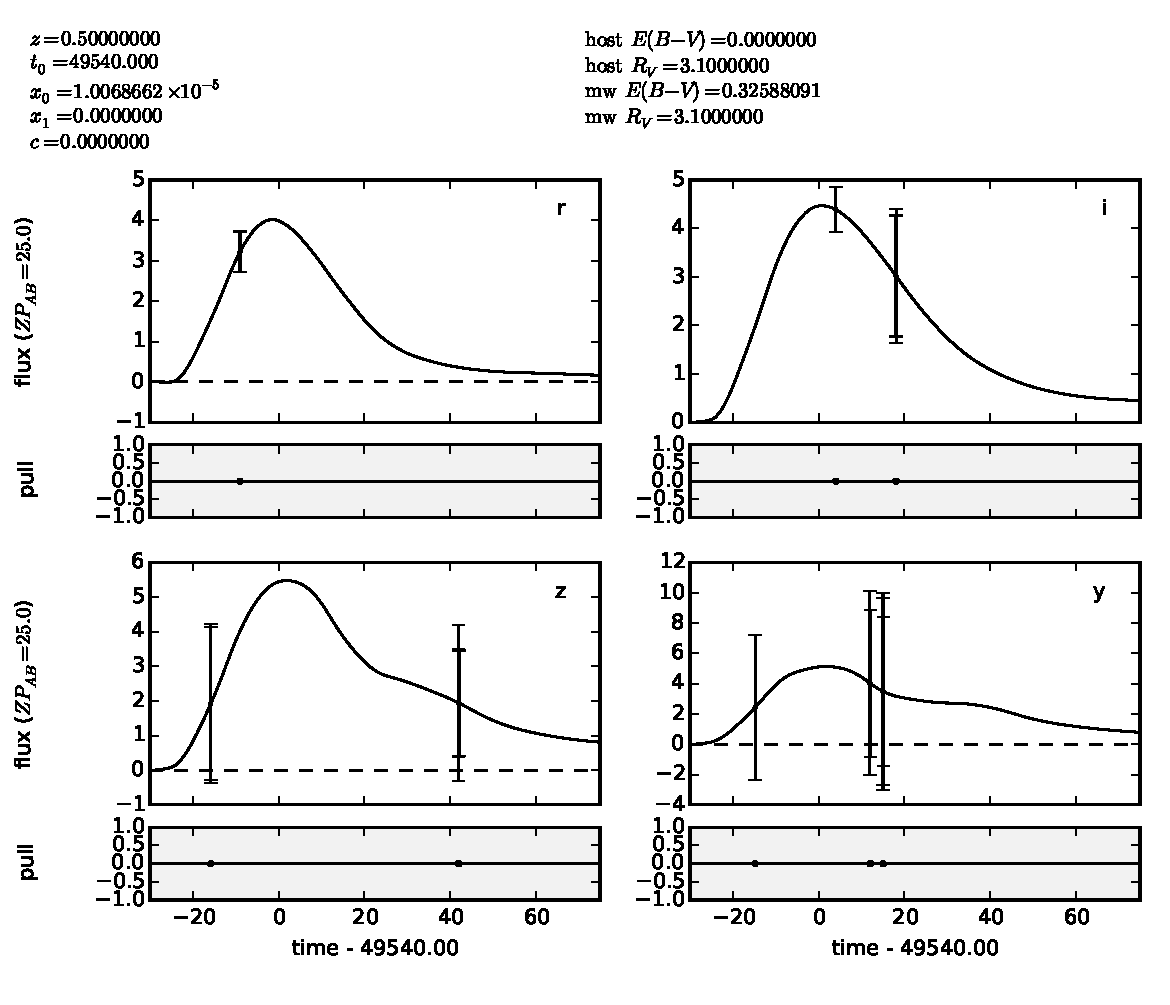
\includegraphics[angle=0,width=0.99\hsize:,clip]{figs/SN_309_lc.pdf}
%\vskip -1.3in
\caption{Light curves of Supernova Type Ia generated using Main Survey of the OpSim output in different bands. The number of data points are limited. 
}
\label{fig:SNIaLCopsimmain}
\end{figure}



%OpSim analysis: how good would the default observing strategy be, at
%the time of writing for this science project?



% --------------------------------------------------------------------

{\bf Suggestion of Rolling-Cadence and its OpSim Run}
%\label{sec:keyword:discussion}

Discussion: what risks have been identified? What suggestions could be
made to improve this science project's figure of merit, and mitigate
the identified risks?

{\bf Rolling-Cadence:} As mentioned above, our goal for observing strategy optimized for SN cosmology
is to obtain 7-10 epochs spread over 50 days or so for more than one filter. We suggest to change the filter 
every day and LSST can choose a part of sky which has the best airmass, centered on Zenith.
LSST will observe about 1/3 of visible sky per day (to be confirmed). LSST can observe the same part of sky for 6 days 
with 6 filters, and repeat 9 times for the same field. This observing strategy will result in 54 visits (with 6 different filters) for the same field. We repeat the same for Field 2 which takes another 54 days. Then observe Field 3 for another 54 days.

\begin{figure}[tbh!]
\vskip -1.3in
%\includegraphics[angle=0,width=0.99\hsize:,clip]{figs/SNIaLCopsim.pdf}
\vskip -1.3in
\caption{Predictions of Light curves of Supernova Type Ia using Rolling-Cadence.
}
\label{fig:SNIaLCopsimmainnew}
\end{figure}



\begin{itemize}
\item Intrinsic Dispersion, environmental effects, newer analysis methods
\item Follow-up procedures: What is feasible? Where will our training samples for classification and light curve models come from (other experiments, our own 
sub-samples with spectroscopic follow-up?), spectroscopic follow-up of host galaxies. Can hosts be identified?
\item `Systematics': In what ways will the real data not match the assumptions made in analysis. Having a large sample of SN, to understand the astrophysics would be useful for this. 
\end{itemize}


% ====================================================================

\navigationbar


% --------------------------------------------------------------------

% ====================================================================
%+
% SECTION NAME:
%    lenstimedelays.tex
%
% CHAPTER:
%    cosmology.tex
%
% ELEVATOR PITCH:
%    Lensed quasars and supernovae provide distance measurements for
%    cosmology. They are a few days to a few weeks in length. To
%    measure them well we need long campaigns (>~3 years) with high
%    night-to-night cadence (better than the standard 5 days if
%    possible, especially as combining all filters might be difficult.)
%
% AUTHORS:
%   Phil Marshall (@drphilmarshall)
%-
% ====================================================================

\section{ Strong Gravitational Lens Time Delays }
\def\secname{lenstimedelays}\label{sec:\secname}

\credit{drphilmarshall},
\credit{rhiannonlynne},
\credit{tanguita}

The multiple images of strongly lensed quasars and supernovae have
delayed arrival times: variability in the first image will be observed
in the second image some time later, as the photons take different
paths around the deflector galaxy, and through different depths of
gravitational potential. If the lens mass distribution can be modeled
independently, using a combination of high resolution imaging of the
distorted quasar/SN host galaxy and stellar dynamics in the lens
galaxy, the measured time delays can be used to infer the ``time delay
distance'' in the system. This distance enables a direct measurement
of the Hubble constant, independent of the distance ladder.

% --------------------------------------------------------------------

\subsection{Target measurements and discoveries}
\label{sec:\secname:targets}

For this cosmological probe to be competitive with LSST's others, the
time delays of several hundred systems (which will be distributed
uniformly over the extragalactic sky) will need to be measured with
bias below the sub-percent level, while the precision required is a
few percent per lens.  In galaxy-scale lenses, the kind that are most
accurately modeled, these time delays are typically between several
days and several weeks long, and so are measurable in monitoring
campaigns having night-to-night cadence of between one and a few days,
and seasons lasting several months or more.

To obtain accurate as well as precise lensed quasar time delays, several
monitoring seasons are required. Lensed supernova time delays have not
yet been measured, but their transient nature means that their time
delay measurements may be more sensitive to cadence than season or
campaign length.

% --------------------------------------------------------------------

\subsection{Metrics}
\label{sec:\secname:metrics}

Anticipating that the time delay accuracy would depend on night-to-night
cadence, season length, and campaign length, we carried out a large
scale simulation and measurement program that coarsely sampled these
schedule properties. In \citet{LiaoEtal2015}, we simulated 5 different
light curve datasets, each containing 1000 lenses, and presented them to
the strong lensing community in a ``Time Delay Challenge.'' These 5
challenge ``rungs'' differed by their schedule properties, in the ways
shown in \autoref{tab:tdcrungs}. Focusing on the best challenge
submissions made by the community, we derived a simple power law model
for the variation of each of the time delay accuracy, time delay
precision, and useable sample fraction, with the schedule properties
cadence, season length and campaign length. These models are shown in
\autoref{fig:tdcresults}, reproduced from \citet{LiaoEtal2015}, and are
given by the following equations:
\begin{align}
|A|_{\rm model} &\approx 0.06\% \left(\frac{\rm cad} {\rm 3 days}  \right)^{0.0}
                          \left(\frac{\rm sea}  {\rm 4 months}\right)^{-1.0}
                          \left(\frac{\rm camp}{\rm 5 years} \right)^{-1.1} \notag \\
  P_{\rm model} &\approx 4.0\% \left(\frac{\rm cad} {\rm 3 days}  \right)^{ 0.7}
                         \left(\frac{\rm sea}  {\rm 4 months}\right)^{-0.3}
                         \left(\frac{\rm camp}{\rm 5 years} \right)^{-0.6} \notag \\
  f_{\rm model} &\approx 30\% \left(\frac{\rm cad} {\rm 3 days}  \right)^{-0.4}
                        \left(\frac{\rm sea}  {\rm 4 months}\right)^{ 0.8}
                        \left(\frac{\rm camp}{\rm 5 years} \right)^{-0.2} \notag
\end{align}

%%%%%%%%%%%%%%%%%%%%%%%%%%%%%%%%%%%%
\begin{table*}
\begin{center}
\capstart
\begin{tabular}{cccccc} \hline\hline
  Rung &  Mean Cadence & Cadence Dispersion & Season   & Campaign & Length   \\
       &  (days)       & (days)             & (months) & (years)  & (epochs) \\ \hline
  0    &    3.0        &   1.0              &   8.0    &    5     & 400      \\
  1    &    3.0        &   1.0              &   4.0    &    10    & 400      \\
  2    &    3.0        &   0.0              &   4.0    &    5     & 200      \\
  3    &    3.0        &   1.0              &   4.0    &    5     & 200      \\
  4    &    6.0        &   1.0              &   4.0    &    10    & 200      \\
\hline\hline
\end{tabular}
\end{center}
\caption{The observing parameters for the five rungs of the Time Delay
Challenge. Reproduced from \citet{LiaoEtal2015}.\label{tab:tdcrungs}}
\end{table*}
%%%%%%%%%%%%%%%%%%%%%%%%%%%%%%%%%%%%

%%%%%%%%%%%%%%%%%%%%%%%%%%%%%%%%%%%
\begin{figure*}[!ht]
  \capstart
  \begin{minipage}[b]{\linewidth}
    \begin{minipage}[b]{0.32\linewidth}
      \centering\includegraphics[width=\linewidth]{figs/Accuracy_season_nca.pdf}
    \end{minipage} \hfill
    \begin{minipage}[b]{0.32\linewidth}
      \centering\includegraphics[width=\linewidth]{figs/Precision_cadence_nca.pdf}
    \end{minipage} \hfill
    \begin{minipage}[b]{0.32\linewidth}
      \centering\includegraphics[width=\linewidth]{figs/Fraction_season_nca.pdf}
    \end{minipage}
  \end{minipage}
\caption{Examples of changes in accuracy $A$ (left), precision $P$
(center) and success fraction $f$ (right) with schedule properties, as
seen in the different TDC submissions. The gray approximate power law
model was derived by visual inspection of the pyCS-SPL results; the
signs of the indices were pre-determined according to our expectations.
Reproduced from \citet{LiaoEtal2015}.}
\label{fig:tdcresults}
\end{figure*}
%%%%%%%%%%%%%%%%%%%%%%%%%%%%%%%%%%%

All three of these metrics would, in an ideal world, be optimized:
this could be achieved by decreasing the night-to-night cadence (to
better sample the light curves), extending the observing season length
(to maximize the chances of capturing a strong variation and its
echo), and extending the campaign length (to increase the number of
effective time delay measurements). A combined figure of merit should
therefore be readily available.

The quantity of greatest scientific interest is the {\it accuracy in
cosmological parameters}: this coudl be computed as follows. Setting a
required accuracy threshold  defines the available number of lenses,
which in turns gives us the mean precision per lens there. Combining the
whole sample, we would get the error on the weighted mean time delay,
and can equate that to the statistical uncertainty on the Hubble
constant. The Figure of merit would be the final precision on $H_0$, as
a way to sum up the sample size and time delay measurability (at fixed
accuracy requirement).

% --------------------------------------------------------------------

\subsection{\OpSim Analysis}
\label{sec:\secname:analysis}

% \OpSim analysis: how good would the default observing strategy be, at
% the time of writing for this science project?

In this section we present the results of our ongoing \OpSim / MAF
analysis, as we try to
answer the question ``how good would the proposed observing
strategies be, for time delay lens cosmography?''

We used the
\simsMAFcontrib{SeasonStacker}{mafContrib/seasonStacker.py} to work
with seasons, rather than calendar years.
We used \texttt{ops2\_1075} \OpSim run for most of our tests, but plan
to re-run on \opsimdbref{db:baseCadence} and
\opsimdbref{db:NoVisitPairs}, in order to assess the new baseline
cadence and compare it against a simulated observing strategy where
the visit pair requirement is relaxed.

% \todo{PJM}{Correct the above paragraphs and add more links to MAF code.}

\autoref{fig:lenstimedelays:results} shows the results of our MAF
analysis of one \OpSim database, \texttt{ops2\_1075}, where we have
assumed that all filters were able to be used in the light curve
analysis (as was implicitly assumed when applying the results of
\citeauthor{LiaoEtal2015}). These sky maps show that, over the main
(WDF) survey area, the time delay accuracy, time delay precision and
time delay lens success fraction are consistently maintained,
indicating that the global average values of these metrics could
conceivably used as higher level metrics or even figure of merit.

% \autoref{tab:lenstimedelays:results} shows the global (i.e. all-sky)
% average values of our metrics, for two different \OpSim
% databases and two different filter set assumptions.
% \todo{PJM}{Compute global average lens time delay metrics and discuss.}
% \todo{PJM}{Define overall figure of merit and compute.}



%%%%%%%%%%%%%%%%%%%%%%%%%%%%%%%%%%%
\begin{figure*}[!ht]
  \capstart
  \begin{minipage}[b]{\linewidth}
    \begin{minipage}[b]{0.32\linewidth}
      \centering\includegraphics[width=\linewidth]{figs/lenstimedelays-ops2_1075-Accuracy-skymap.png}
    \end{minipage} \hfill
    \begin{minipage}[b]{0.32\linewidth}
      \centering\includegraphics[width=\linewidth]{figs/lenstimedelays-ops2_1075-Precision-skymap.png}
    \end{minipage} \hfill
    \begin{minipage}[b]{0.32\linewidth}
      \centering\includegraphics[width=\linewidth]{figs/lenstimedelays-ops2_1075-Fraction-skymap.png}
    \end{minipage}
  \end{minipage}
\caption{Sky maps of the accuracy $A$ (left), precision $P$ (center) and
success fraction $f$ (right) metrics, for the \texttt{ops2\_1075} \OpSim
database and assuming all filters ($ugrizy$) are used in the analysis
according to the assumptions described in the text.}
\label{fig:lenstimedelays:results}
\end{figure*}
%%%%%%%%%%%%%%%%%%%%%%%%%%%%%%%%%%%


% %%%%%%%%%%%%%%%%%%%%%%%%%%
% \begin{table*}
% \begin{center}
% \caption{Lens Time Delay Metric Analysis Results.}
% \label{tab:lenstimedelays:results}
% \footnotesize
% \begin{tabularx}{\linewidth}{ccccccccc}
%   \hline
%   \OpSim run
%    & Filters
%     & \texttt{cadence}
%      & \texttt{season}
%       & \texttt{campaign}
%        & \texttt{Accuracy}
%         & \texttt{Precision}
%          & \texttt{Fraction}
%           & \texttt{timedelayFoM} \\
%   \hline\hline
%
%   \opsimdbref{db:baseCadence}
%    & $ri$
%     & $XXX$
%      & $XXX$
%       & $XXX$
%        & $XXX$
%         & $XXX$
%          & $XXX$
%           & ??? \\
%
%   \opsimdbref{db:baseCadence}
%    & $ugrizy$
%     & $XXX$
%      & $XXX$
%       & $XXX$
%        & $XXX$
%         & $XXX$
%          & $XXX$
%           & ??? \\
%   \hline
%
%   \opsimdbref{db:NoVisitPairs}
%    & $ri$
%     & $XXX$
%      & $XXX$
%       & $XXX$
%        & $XXX$
%         & $XXX$
%          & $XXX$
%           & ??? \\
%
%   \opsimdbref{db:NoVisitPairs}
%    & $ugrizy$
%     & $XXX$
%      & $XXX$
%       & $XXX$
%        & $XXX$
%         & $XXX$
%          & $XXX$
%           & ??? \\
%   \hline
%
% \multicolumn{9}{p{\linewidth}}{\scriptsize Notes: see the text for
% the definitions of each metric, and sky maps and histogram
% plots of them. The Figure of Merit is still under development.}
% \end{tabularx}
% \normalsize
% \medskip\\
% \end{center}
% \end{table*}
% %%%%%%%%%%%%%%%%%%%%%%%%%%
%

% --------------------------------------------------------------------

\subsection{Discussion}
\label{sec:\secname:discussion}

% \todo{PJM}{Write lens time delays discussion section.}

The main risk involved with this science case
is that the multi-filter light curve analysis will not be well approximated by
the real-life combination of all 6 filters together.
The second time delay challenge (TDC2) will help answer this
question.  For now, just using 2 filters gives a lower limit on the
overall precision we should expect.

We would expect the relaxation of the visit pairs requirement to
increase the  night to night cadence by a factor of two, if the visits
are redistributed randomly in time. If \OpSim is not being as liberal as
this, we may not see much improvement over the baseline cadence:
efficiency maximization could be preventing visits being fully split. We
are interested in any changes to the WFD survey time sampling that
reduce the inter-night gaps: these  would include rolling cadence
schemes.

% Also need to assess 1 vs 3 vs 10 year light curves. How do metrics
% improve? What will be possible in the early part of the survey?

% ====================================================================
%
% \subsection{Conclusions}
%
% Here we answer the ten questions posed in
% \autoref{sec:intro:evaluation:caseConclusions}:
%
% \begin{description}
%
% \item[Q1:] {\it Does the science case place any constraints on the
% tradeoff between the sky coverage and coadded depth? For example, should
% the sky coverage be maximized (to $\sim$30,000 deg$^2$, as e.g., in
% Pan-STARRS) or the number of detected galaxies (the current baseline but
% with 18,000 deg$^2$)?}
%
% \item[A1:] ...
%
% \item[Q2:] {\it Does the science case place any constraints on the
% tradeoff between uniformity of sampling and frequency of  sampling? For
% example, a rolling cadence can provide enhanced sample rates over a part
% of the survey or the entire survey for a designated time at the cost of
% reduced sample rate the rest of the time (while maintaining the nominal
% total visit counts).}
%
% \item[A2:] ...
%
% \item[Q3:] {\it Does the science case place any constraints on the
% tradeoff between the single-visit depth and the number of visits
% (especially in the $u$-band where longer exposures would minimize the
% impact of the readout noise)?}
%
% \item[A3:] ...
%
% \item[Q4:] {\it Does the science case place any constraints on the
% Galactic plane coverage (spatial coverage, temporal sampling, visits per
% band)?}
%
% \item[A4:] ...
%
% \item[Q5:] {\it Does the science case place any constraints on the
% fraction of observing time allocated to each band?}
%
% \item[A5:] ...
%
% \item[Q6:] {\it Does the science case place any constraints on the
% cadence for deep drilling fields?}
%
% \item[A6:] ...
%
% \item[Q7:] {\it Assuming two visits per night, would the science case
% benefit if they are obtained in the same band or not?}
%
% \item[A7:] ...
%
% \item[Q8:] {\it Will the case science benefit from a special cadence
% prescription during commissioning or early in the survey, such as:
% acquiring a full 10-year count of visits for a small area (either in all
% the bands or in a  selected set); a greatly enhanced cadence for a small
% area?}
%
% \item[A8:] ...
%
% \item[Q9:] {\it Does the science case place any constraints on the
% sampling of observing conditions (e.g., seeing, dark sky, airmass),
% possibly as a function of band, etc.?}
%
% \item[A9:] ...
%
% \item[Q10:] {\it Does the case have science drivers that would require
% real-time exposure time optimization to obtain nearly constant
% single-visit limiting depth?}
%
% \item[A10:] ...
%
% \end{description}

\navigationbar

% ====================================================================


% --------------------------------------------------------------------
